\subsubsection{Descrizione generale}
Questo servizio implementa le funzionalità di scraping ed in generale ottenimento dati da Instagram e altre piattaforme ad esso correlate.

\subsubsection{Diagramma delle classi}
\begin{figure}[H]
    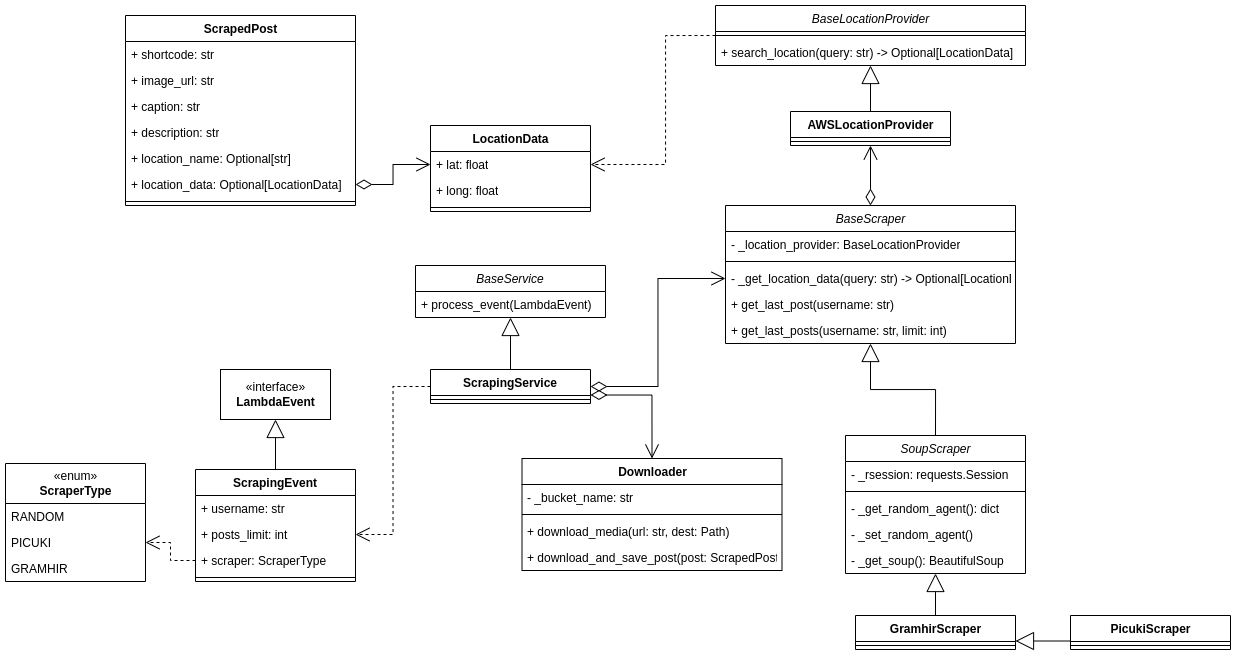
\includegraphics[width=14cm]{sezioni/images/cd_scraping.png}
    \centering
    \caption{Scraping Service - Diagramma delle classi}
\end{figure}

\subsubsection{Schemi I/O}
\paragraph*{Input} esempio di evento in input, in formato JSON\G{}.
\begin{lstlisting}[language=JSON]
{
    "username": "antoniorazzi",
    "posts_limit": 10
}
\end{lstlisting}
Descrizione:
\begin{itemize}
    \item \verb|username|: username del profilo social da cui effettuare lo scraping;
    \item \verb|posts_limit|: numero massimo di post di cui effettuare lo scraping. 
\end{itemize}

\paragraph*{Output} esempio di risposta in output, in formato JSON\G{}.
\begin{lstlisting}[language=JSON]
{
    "posts_count": 2,
    "posts": [
        {"id": 4},
        {"id": 5}
    ]
}
\end{lstlisting}
Descrizione:
\begin{itemize}
    \item \verb|posts_count|: numero di post ottenuti;
    \item \verb|posts|: array di post. 
\end{itemize}

\subsubsection{Strategie di scraping}
Le azioni di scraping non avvengono direttamente su Instagram, questo perchè comporterebbe il
rischio di incorrere in \textit{rate limiting} o addirittura l'impossibilità totale di usufruire del servizio dall'infrastruttura cloud di AWS.
Per aggirare queste problematiche, lo scraping avviene da piattaforme chiamate \textit{viewer},
che propongono in larga parte gli stessi contenuti di Instagram, ma in un formato molto più semplice da trattare automaticamente.\aCapo
Le classi \verb|SoupScraper| e più in generale \verb|BaseScraper|, si occupano di fornire interfacce comuni per gli scraper che andranno implementati.
Le classi \verb|GramhirScraper| e \verb|PicukiScraper| si occupano di effettuare lo scraping 
rispettivamente dai viewer \textit{Gramhir} (\url{https://www.gramhir.com}) e \textit{Picuki} (\url{https://www.picuki.com}). Gli algoritmi e le tecniche utilizzate dalle due classi, sono sostanzialmente identiche.
Infatti, \verb|PicukiScraper| eredita direttamente da \verb|GramhirScraper|.
Il funzionamento interno delle due piattaforme differisce solo nella necessità di ottenere un 
\textit{ID} correlato al profilo social che si vuole visualizzare, necessario per \textit{Gramhir}.

\begin{lstlisting}[language=Python, caption=Ottenimento URL profilo in \textit{Gramhir}]
def _get_profile_url(self, username: str) -> str:
    gramhir_id = self._get_profile_internal_id(username)
    profile_url = self._PROFILE_URL.format(username=username, gramhir_id=gramhir_id)
    return profile_url
\end{lstlisting}

\begin{lstlisting}[language=Python, caption=Ottenimento URL profilo in \textit{Picuki}]
def _get_profile_url(self, username: str) -> str:
    return self._PROFILE_URL.format(username=username)
\end{lstlisting}

Lo scraping vero e proprio avviene tramite parsing\G{} del contenuto HTML\G{} delle pagine web
fornite dai \textit{viewer}.

\subsubsection{Salvataggio dei dati}
I dati relativi ai post ottenuti e le relative posizioni, vengonono salvati nel database.
Le immagini o altri contenuti multimediali vengonono salvati nell'apposito bucket in S3.
